\documentclass[a4paper,12pt]{article}

\usepackage{abakos}
\usepackage[brazilian,english]{babel}
\usepackage[utf8]{inputenc}
\usepackage[T1]{fontenc}
\usepackage{abntex2cite}
\usepackage{graphicx}
\usepackage{float}
\usepackage{url}
\usepackage{setspace}
\usepackage{amsmath}
\usepackage{amssymb}
\usepackage{array}
\usepackage{tabularx}
\usepackage{tikz}
\usetikzlibrary{shapes.geometric,arrows.meta,positioning}
\setlength{\headheight}{22.4pt}

\newcolumntype{Y}{>{\raggedright\arraybackslash}X}
\newcolumntype{P}[1]{>{\raggedright\arraybackslash}p{#1}}
\newcolumntype{C}{>{\centering\arraybackslash}X}

% Marca de referência ainda não incluída em bibliografia.bib (localizar e conferir antes da submissão)
\newcommand{\refnec}{[REFERÊNCIA NECESSÁRIA]}

%%%%%%%%%%%%%%%%%%%%%%%%%%%
% Capa da revista
%%%%%%%%%%%%%%%%%%%%%%%%%%

\newcommand{\monog}{Previsão de Carga Computacional de Curto Prazo para Estimativa da Demanda Energética de TI em Datacenters: Um Estudo com o Alibaba Cluster Trace}
\newcommand{\monogES}{Short-Term Computational Workload Forecasting for IT Energy Demand Estimation in Datacenters: A Study Using the Alibaba Cluster Trace}
\newcommand{\origem}{Brasil}
\newcommand{\editorial}{\textbf{Abakós}, Belo Horizonte, v. 14, n. 1, p. 00-00, Maio 2026 - ISSN: 2316-9451}

%%%%%%%%%%%%%%%%% INFORMAÇÕES SOBRE AUTORES %%%%%%%%%%%%%%%%%%%%%%%%%%%%%%%

\newcommand{\AutorA}{Jorge Inácio de Oliveira}
\newcommand{\funcaoA}{Bacharelando em Engenharia de Computação}
\newcommand{\cursA}{Instituto de Ciências Exatas e de Informática da PUC Minas}
\newcommand{\emailA}{jorge.oliveira@sga.pucminas.br}

\newcommand{\AutorB}{Leonardo Piuzana Pizani}
\newcommand{\funcaoB}{Bacharelando em Engenharia de Computação}
\newcommand{\cursB}{Instituto de Ciências Exatas e de Informática da PUC Minas}
\newcommand{\emailB}{leonardo.pizani@sga.pucminas.br}

\newcommand{\AutorC}{Lucas José de Freitas}
\newcommand{\funcaoC}{Bacharelando em Engenharia de Computação}
\newcommand{\cursC}{Instituto de Ciências Exatas e de Informática da PUC Minas}
\newcommand{\emailC}{ljfreitas@sga.pucminas.br}

\newcommand{\AutorD}{Tiago Carvalho Moscoso}
\newcommand{\funcaoD}{Bacharelando em Engenharia de Computação}
\newcommand{\cursD}{Instituto de Ciências Exatas e de Informática da PUC Minas}
\newcommand{\emailD}{tiago.moscoso@sga.pucminas.br}

\newcommand{\AutorE}{Natalia Camillo do Carmo}
\newcommand{\funcaoE}{Orientadora. Mestre em Ciência da Computação}
\newcommand{\cursE}{Instituto de Ciências Exatas e de Informática da PUC Minas}
\newcommand{\emailE}{nataliacarmo@pucminas.edu.br}

\newcommand{\keyword}[1]{\textsf{#1}}

\begin{document}

%%%%%%%%%%%%%%%%%%%%%%%%%%%%%%%%%%
%% Pagina de titulo
%%%%%%%%%%%%%%%%%%%%%%%%%%%%%%%%%%

\begin{flushleft}
\begin{minipage} [c][5cm][b]{16.5cm}

\includegraphics[scale=1.1]{figuras/pucmg.png}
\end{minipage}
 \vspace{0cm} {
 \singlespacing \Large{\monog \symbolfootnote[1]{Submetido em 26/03/2026} \\ }
  \normalsize{\monogES}
 }
\end{flushleft}

\begin{flushright}
\singlespacing
\normalsize{\AutorA \footnote{\funcaoA. \cursA, \origem. E-mail: \emailA }} \\
\normalsize{\AutorB \footnote{\funcaoB. \cursB, \origem. E-mail: \emailB }} \\
\normalsize{\AutorC \footnote{\funcaoC. \cursC, \origem. E-mail: \emailC }} \\
\normalsize{\AutorD \footnote{\funcaoD. \cursD, \origem. E-mail: \emailD }} \\
\normalsize{\AutorE \footnote{\funcaoE. \cursE, \origem. E-mail: \emailE }} \\
\end{flushright}
\thispagestyle{empty}

\begin{abstract}
\noindent
O crescimento de aplicações de Inteligência Artificial aumentou o consumo energético dos \textit{datacenters}. Este trabalho avaliou a previsão de curto prazo (5 a 30~min) da utilização agregada de CPU das 4.023 máquinas do \textit{Alibaba Cluster Trace} v2018 e a propagação do seu erro para a energia de TI estimada por um modelo paramétrico de potência com servidores substitutos do SPECpower\_ssj2008, já que o \textit{trace} não tem medição elétrica. Foram comparados persistência, Ridge, XGBoost, modelos de espaço de estados, cinco redes neurais, previsão hierárquica por grupos de máquinas, um modelo global por máquina, combinação por regime e quantis calibrados, sob validação temporal com purga, um teste de 24~h e uma avaliação pré-registrada em quatro dias. O XGBoost com defasagens, médias móveis e calendário superou a persistência com significância em 5~min, e nenhum modelo o superou após a correção de Holm. As redes tiveram viés ligado ao deslocamento de nível entre treino e avaliação, e todos os modelos subestimaram os picos. A calibração adaptativa levou a cobertura do limite de 95\% a 0,95. O erro de energia modelada ficou entre 2,3\% e 6,1\% por janela, e aplicar a curva de potência à CPU média superestimou a energia em 1,2\%, efeito reduzido pela modelagem por grupos de máquinas.
\\\textbf{\keyword{Palavras-chave: }} Eficiência Energética. Datacenters. Inteligência Artificial. Previsão de Carga Computacional.
\end{abstract}

%%%%%%%%%%%%%%%%%%%%%%%%%%%%%%%%%%%%%%%%%%%%%%%%%%%%%%%%%
\newpage
\selectlanguage{english}
\begin{abstract}
\noindent
The growth of Artificial Intelligence applications has increased the energy use of datacenters. This work evaluated short-term forecasting (5 to 30~min) of the aggregate CPU utilization of the 4,023 machines in the \textit{Alibaba Cluster Trace} v2018 and the propagation of its error into the IT energy estimated by a parametric power model with substitute servers from SPECpower\_ssj2008, since the trace contains no electrical measurements. Persistence, Ridge, XGBoost, state-space models, five neural networks, hierarchical forecasting over machine groups, a global per-machine model, regime-based combination, and calibrated quantiles were compared under time-ordered validation with purging, a 24-hour test, and a pre-registered evaluation over four days. XGBoost with lags, moving averages, and calendar features outperformed persistence significantly at 5~min, and no model outperformed it after Holm correction. The neural networks showed a bias tied to the level shift between training and evaluation, and all models underestimated peaks. Adaptive calibration brought the coverage of the 95\% bound to 0.95. The modeled energy error ranged from 2.3\% to 6.1\% per window, and applying the power curve to the mean CPU overestimated energy by 1.2\%, an effect reduced by modeling groups of machines.
\\\textbf{\keyword{Keywords: }} Energy Efficiency. Datacenters. Artificial Intelligence. Workload Prediction.
\end{abstract}

\newpage

\selectlanguage{brazilian}
 \onehalfspace
 \setlength{\parindent}{1.25cm}

%%%%%%%%%%%%%%%%%%%%%%%%%%%%%%%%%%%%%%%%%%%%%%%%%
%% 1. INTRODUÇÃO
%%%%%%%%%%%%%%%%%%%%%%%%%%%%%%%%%%%%%%%%%%%%%%%%%

\section{Introdução}

\subsection{Contextualização e Motivação}

Os centros de processamento de dados (\textit{datacenters}) evoluíram de salas de servidores isoladas para infraestruturas globais que sustentam a economia digital, e a expansão da computação em nuvem e da Inteligência Artificial (IA) acelerou sua densidade computacional. O consumo elétrico tornou-se um desafio de primeira ordem: estimativas da literatura apontam entre 1\% e 3\% do consumo mundial de eletricidade, com crescimento associado a cargas de IA generativa \cite{shaffi2026}.

O problema técnico está na dinâmica das cargas de trabalho (\textit{workloads}). Resfriamento e distribuição de energia são frequentemente dimensionados para o pico, o que gera desperdício quando o processamento está baixo e afasta o \textit{Power Usage Effectiveness} (PUE) do ideal de 1,0 (Seção~\ref{sec:pue-teorico}). Prever a carga computacional de curto prazo e traduzi-la em demanda elétrica de TI é um passo para apoiar esse planejamento com dados.

\subsection{Objetivos}

\subsubsection{Objetivo geral}

O objetivo geral deste trabalho foi desenvolver e avaliar um \textit{pipeline} reprodutível de previsão da utilização futura de CPU de curto prazo e de estimativa da demanda energética de TI associada, com base em métricas operacionais reais do \textit{Alibaba Cluster Trace} v2018 e em um modelo paramétrico de potência parametrizado por dados públicos de \textit{benchmark}, comparando algoritmos de complexidade crescente em múltiplos horizontes.

\subsubsection{Objetivos específicos}

Como objetivos específicos, buscou-se:

\begin{itemize}
    \item caracterizar a série agregada de CPU do \textit{trace} e as séries de memória, rede e disco;
    \item construir atributos temporais (defasagens, estatísticas móveis e calendário) com prevenção explícita de vazamento de dados;
    \item comparar persistência, Ridge, XGBoost, modelos residuais e de espaço de estados e redes neurais sequenciais na previsão direta em 5, 15 e 30~min, e avaliar por ablação o efeito das variáveis exógenas;
    \item verificar se a estrutura por máquina (previsão hierárquica e modelo global) e a combinação de previsores melhoram a previsão do agregado;
    \item avaliar os modelos por MAE, RMSE e MASE, erro nos picos e inferência por \textit{block bootstrap}, e estimar limites superiores por quantis calibrados;
    \item estimar a energia de TI com o modelo de potência de \citeonline{fan2007power} parametrizado pelo SPECpower\_ssj2008, quantificar a propagação do erro de previsão e o efeito de agregar a utilização antes da curva de potência;
    \item documentar o \textit{pipeline} de forma reprodutível, com código versionado e sementes fixas.
\end{itemize}

\subsection{Justificativa}

A energia elétrica pesa nos custos operacionais de \textit{datacenters} \cite{gao2014}, e as emissões indiretas do consumo elétrico respondem por mais de 90\% do impacto ambiental da refrigeração \cite{erkek2026}. Exigências regulatórias e de governança ESG tornam a gestão do consumo uma demanda concreta \cite{zatonatska2024comprehensive}: na União Europeia, a \citeonline{eu2024reg1364} obriga operadores com potência de TI instalada de pelo menos 500~kW a reportar indicadores de sustentabilidade, entre eles o PUE, previstos no Artigo 12 da \citeonline{eu2023directive1791}. Modelos que estimem a demanda de TI a partir da carga apoiam decisões de capacidade, de alocação e de viabilidade. Este trabalho contribui com uma avaliação em dados de produção que separa explicitamente a previsão de carga, aprendida dos dados, da estimativa de energia, modelada.

\subsection{Problema de pesquisa}

Parte significativa da literatura valida propostas apenas em simulação \cite{kahil2025} (Seção~\ref{sec:trabalhos-correlatos}), e a base pública adotada aqui não traz medição elétrica (Seção~\ref{sec:dados}). O trabalho foi orientado pela questão: \textit{em que medida modelos de Inteligência Artificial de complexidade crescente preveem a utilização futura de CPU de curto prazo em um cluster de produção (Alibaba Cluster Trace v2018) com erro inferior ao de baselines ingênuos, e como esse erro se propaga para a demanda energética de TI estimada por um modelo paramétrico de potência?}

\subsection{Escopo e delimitações}

O escopo limitou-se à previsão da utilização de CPU a partir de métricas operacionais reais e à estimativa, não à medição, da energia de TI associada. Não foram abordados projeto físico, sistemas reais de refrigeração nem controle de equipamentos. Com passo de 300~s e horizontes de 5 a 30~min, a previsão atende ao planejamento de capacidade de curto prazo, não a decisões em milissegundos. O PUE não foi calculado, porque o \textit{trace} não contém a energia total da instalação.

\subsection{Organização do trabalho}

A Seção~2 apresenta o referencial teórico e os trabalhos correlatos. A Seção~3 descreve os dados, o protocolo de avaliação, os modelos, o modelo de potência e os critérios estatísticos. A Seção~4 apresenta os resultados: caracterização dos dados, comparação de modelos, inferência, picos, previsão probabilística e energia. A Seção~5 discute os resultados e as limitações, e a Seção~6 conclui.

%%%%%%%%%%%%%%%%%%%%%%%%%%%%%%%%%%%%%%%%%%%%%%%%%
%% 2. REFERENCIAL TEÓRICO
%%%%%%%%%%%%%%%%%%%%%%%%%%%%%%%%%%%%%%%%%%%%%%%%%

\section{Referencial Teórico}

\subsection{Eficiência Energética em Datacenters}

A eficiência energética em \textit{datacenters} envolve servidores, resfriamento, distribuição elétrica e rede. \citeonline{patel2025artificial} destaca que algoritmos treinados com dados de sensores podem antecipar demandas e reduzir desperdício em resfriamento e na alocação de cargas, com reduções entre 20\% e 35\% na energia de resfriamento e melhora de 0,15 a 0,25 no PUE em implementações industriais específicas, em condições distintas das deste trabalho.

\subsection{Power Usage Effectiveness (PUE)}
\label{sec:pue-teorico}

O PUE é a razão entre a energia total da instalação e a energia dos equipamentos de TI:

\begin{equation}
    \mathrm{PUE} = \frac{E_{\mathrm{total}}}{E_{\mathrm{TI}}}.
    \label{eq:pue}
\end{equation}

\noindent O valor ideal é 1,0; na prática os valores ficam acima disso, com registros superiores a 2,2 reduzidos para cerca de 1,48 por modernizações \cite{song2026}. O PUE e suas componentes podem ser previstos com dados operacionais: \citeonline{gao2014} estimam o PUE no Google com rede neural e erro absoluto médio de 0,004; \citeonline{zhang2022} preveem o PUE anual a partir de variáveis climáticas; e \citeonline{cho2025} mostram que o resfriamento é determinante central do indicador num \textit{datacenter} de 30~MW voltado a IA. Neste trabalho, o PUE situa o problema: o \textit{pipeline} estima o denominador $E_{\mathrm{TI}}$ da Equação~\eqref{eq:pue}, sem medir $E_{\mathrm{total}}$. Quando a base não traz medição elétrica, a potência associada à utilização é obtida por modelo paramétrico; \citeonline{fan2007power} propõem um modelo linear e um empírico não linear, este adotado aqui (Seção~\ref{sec:modelo-potencia}).

\subsection{Aprendizado de Máquina Aplicado à Predição Energética}

Abordagens baseadas em limiares rígidos reagem depois da variação do sistema e não capturam relações não lineares entre carga, energia e temperatura \cite{kahil2025,gao2014}. Na predição de consumo de resfriamento, \citeonline{sulaiman2025cnn} obtêm $R^2$ de 0,9435 com CNN-LSTM, e \citeonline{zhou2025load} alcançam $R^2$ superior a 0,9982 numa estrutura hierárquica que integra computação, resfriamento e energia. Em ambiente real, \citeonline{veigas2025digital} aplicam LightGBM à predição de temperatura e consumo de um cluster HPC; em simulação, \citeonline{jonnalagadda2025ai} reportam MAE de 2,1 para redes neurais contra 3,4 para regressão. \citeonline{11470282} detectam anomalias de consumo com um \textit{autoencoder} sobre versões de GPU do \textit{Alibaba Cluster Trace}, com acurácia de 0,9453.

\subsection{Previsão de Carga e Gestão Energética em Clusters}

\citeonline{zhu2019attention} propõem uma LSTM \textit{encoder-decoder} com atenção validada sobre o \textit{Alibaba Cluster Trace}, evidência que motivou a inclusão de modelos sequenciais neste trabalho. \citeonline{zhai2025} usam LSTM sobre o mesmo \textit{trace} (2018) como etapa de um escalonamento orientado ao aproveitamento de energia eólica. Outros trabalhos aplicam previsões a controle: \citeonline{wang2026ea} propõem escalonamento e controle de resfriamento por \textit{Deep Reinforcement Learning} num \textit{datacenter} parcialmente solar, e \citeonline{8885124} combinam LSTM com um agente \textit{Deep Q-Network} para alocação de tarefas, com redução de cerca de 10\% no consumo. Essas decisões estão fora do escopo deste trabalho, que se concentra na previsão e na propagação de seu erro para a energia estimada.

\subsection{Trabalhos Correlatos}
\label{sec:trabalhos-correlatos}

\citeonline{kahil2025} revisam 65 estudos (2019--2024) sobre aprendizado por reforço para otimização energética em \textit{datacenters} e apontam que 95\% validam suas propostas exclusivamente em simulação. \citeonline{xiong2026} combinam SVR com meta-heurísticas (PSO, GWO e ALO) para otimizar hiperparâmetros na predição de consumo, com redução do erro em relação a modelos tradicionais. \citeonline{pannocchi2024} comparam programação linear inteira mista e heurísticas genéticas na alocação de máquinas virtuais, mostrando a interdependência entre alocação computacional e demanda elétrica. A Tabela~\ref{tab:sintese-literatura} sistematiza os trabalhos mais representativos.

\begin{table}[htb]
\caption{Síntese comparativa dos principais trabalhos revisados}
\label{tab:sintese-literatura}
\centering
\scriptsize
\setlength{\tabcolsep}{3pt}
\renewcommand{\arraystretch}{1.05}
\begin{tabularx}{\textwidth}{|P{3.1cm}|P{1.8cm}|Y|P{1.3cm}|P{2.3cm}|}
\hline
\textbf{Referência} & \textbf{Técnica} & \textbf{Variáveis de entrada} & \textbf{Métrica} & \textbf{Resultado} \\
\hline
\cite{gao2014} & MLP (5 camadas) & Carga TI, temperatura, entalpia, bombas & MAE & MAE = 0{,}004 na predição de PUE \\
\hline
\cite{sulaiman2025cnn} & CNN-LSTM-BMO & Temperatura, carga de \textit{chiller} & RMSE, $R^2$ & RMSE = 0{,}5523; $R^2$ = 0{,}9435 \\
\hline
\cite{zhou2025load} & Hierárquico (física + ML) & Computação, resfriamento, energia & $R^2$, erro relativo & $R^2 > 0{,}9982$; erro $< 0{,}63\%$ \\
\hline
\cite{xiong2026} & SVR + meta-heurísticas & Série temporal de consumo & MAE, RMSE & Redução significativa de erro vs.\ modelos tradicionais \\
\hline
\cite{veigas2025digital} & LightGBM (\textit{digital twin}) & CPU, carga térmica, potência & MAE, MAPE & Baixos erros; viável em ambiente HPC real \\
\hline
\cite{jonnalagadda2025ai} & Rede neural profunda vs.\ Regressão & CPU, temperatura, carga, resfriamento & MAE & Rede neural (2{,}1) supera regressão (3{,}4) \\
\hline
\cite{shaffi2026} & XGBoost + MILP & Carga do servidor, temperatura & Custo, renováveis & 59{,}25\% renováveis; 15\% redução de custo \\
\hline
\cite{11470282} & \textit{Autoencoder} robusto & CPU, GPU, rede, memória, disco & Acurácia & 0{,}9453 na detecção de anomalias \\
\hline
\cite{zhu2019attention} & LSTM \textit{encoder-decoder} com atenção & Carga de trabalho (Alibaba/Dinda) & -- & Superior a LSTM convencional na previsão multivariada de carga \\
\hline
\end{tabularx}
\\[0.3cm]
\textbf{\footnotesize Fonte: Autoria própria, com base na literatura revisada.}
\end{table}

As variáveis térmicas recorrentes nesses trabalhos não estão no \textit{Alibaba Cluster Trace}, e os resultados reportados vêm de tarefas e bases diferentes da deste trabalho; eles motivam a progressão de modelos, mas não antecipam qual vencerá na previsão de CPU de um cluster de produção.

%%%%%%%%%%%%%%%%%%%%%%%%%%%%%%%%%%%%%%%%%%%%%%%%%
%% 3. METODOLOGIA
%%%%%%%%%%%%%%%%%%%%%%%%%%%%%%%%%%%%%%%%%%%%%%%%%

\section{Metodologia}

\subsection{Visão Geral da Metodologia}

A pesquisa foi conduzida em etapas sucessivas, cada uma corrigindo limitações da anterior. Um ensaio preliminar de protocolo usou uma série auxiliar de GPU. Em seguida, o protocolo foi aplicado ao \textit{Alibaba Cluster Trace} v2018 com persistência, Ridge e XGBoost como linhas de base e depois ampliado com modelos residuais, de espaço de estados, redes neurais, quantis e o modelo de potência, todos avaliados no mesmo teste final de 24~h. Por fim, o teste único foi substituído por quatro blocos diários de avaliação, que incorporaram a estrutura por máquina e o cálculo da energia por grupos e por máquina. A Figura~\ref{fig:diagrama-metodologia} resume o fluxo; o erro de previsão (fases 3 e 4) é o que se propaga até a energia de TI (fase 5).

\begin{figure}[htb]
\centering
\caption[Diagrama de blocos da metodologia]{Diagrama de blocos da metodologia}
\label{fig:diagrama-metodologia}
\begin{tikzpicture}[
    node distance=0.7cm and 0.6cm,
    fase/.style={rectangle, draw=black, rounded corners=3pt, align=center, text width=4.4cm, minimum height=2.1cm, font=\footnotesize},
    seta/.style={-{Latex[length=2.5mm]}, thick}
]
\node[fase] (dados) {\textbf{1. Dados}\\ \textit{Alibaba Cluster Trace} v2018\\ \textit{machine\_usage}, 4.023 máquinas\\ série agregada e painel por máquina};
\node[fase, right=of dados] (prep) {\textbf{2. Preparação}\\ grade de 300~s\\ defasagens, janelas e calendário\\ \textit{split} temporal com purga};
\node[fase, right=of prep] (mod) {\textbf{3. Modelagem}\\ árvores, espaço de estados, redes\\ hierárquico, global, regimes\\ quantis e calibração conformal};
\node[fase, below=of mod] (aval) {\textbf{4. Avaliação}\\ MAE, RMSE, MASE, picos\\ teste de 24~h e 4 dias\\ \textit{block bootstrap} e Holm};
\node[fase, left=of aval] (ener) {\textbf{5. Energia de TI}\\ modelo de potência $P(u)$\\ servidores SPECpower\\ rotas média, grupo e máquina};
\draw[seta] (dados) -- (prep);
\draw[seta] (prep) -- (mod);
\draw[seta] (mod) -- (aval);
\draw[seta] (aval) -- (ener);
\end{tikzpicture}
\\[0.2cm]
\textbf{\footnotesize Fonte: Autoria própria.}
\end{figure}

\subsection{Dados e Pré-processamento}
\label{sec:dados}

O \textit{Alibaba Cluster Trace} v2018 \cite{alibaba2018clusterdata} registra 4.034 máquinas de um cluster de produção ao longo de 8 dias, em seis tabelas. Serviços online em contêineres e tarefas \textit{batch} são co-localizados nas mesmas máquinas \cite{alibaba2018clusterdata,everman2021cost}, e a utilização de cada máquina é a soma das duas classes. A tabela \textit{machine\_usage} foi a fonte única da variável-alvo (\texttt{cpu\_util\_percent}) e das exógenas (\texttt{mem\_util\_percent}, \texttt{net\_in}, \texttt{net\_out} e \texttt{disk\_io\_percent}), todas normalizadas em [0, 100]; \textit{machine\_meta} forneceu \texttt{cpu\_num} e status. O \textit{trace} não contém potência, energia, temperatura nem GPU \cite{everman2021cost}. A largura de banda de memória (\texttt{mem\_gps}) ficou de fora por estar ausente em 79,3\% das linhas.

A leitura percorreu $246\,934\,820$ linhas. Como os \textit{timestamps} não têm passo predominante, adotou-se uma grade de 300~s, com 2.304 intervalos. A série-alvo é a média da CPU das máquinas presentes em cada intervalo, ponderada por \texttt{cpu\_num}; como todas as máquinas têm \texttt{cpu\_num} igual a 96, a ponderação equivale à média simples. A população principal reúne as 4.023 máquinas com metadado e registro de uso, sem filtro de status; ela inclui uma máquina inativa (\texttt{m\_2739}). Uma coorte só com máquinas ativas (4.022) foi mantida como sensibilidade: as séries diferem em até 0,026 ponto percentual (p.p.), e as métricas são reportadas para a população principal. Valores fora de [0, 100] foram tratados como ausentes. Para a avaliação por blocos diários, construiu-se também um painel por máquina (2.304 intervalos $\times$ 4.023 máquinas), que reproduziu a série agregada com diferença máxima de $1{,}1 \times 10^{-7}$~p.p.

Os atributos foram defasagens de 1, 2, 3, 6 e 12 passos, médias e desvios móveis de 6 e 12 passos e o calendário, codificado por seno e cosseno da posição no ciclo de 24~h do \textit{trace}, que não tem horário civil. Defasagens e janelas terminam na origem $t$, e $u_t$ entra como atributo de todos os modelos. As configurações de ablação foram A (só CPU e calendário), B (A e memória), C (B, rede e disco) e D (A e a distribuição da CPU entre as máquinas na origem).

\subsection{Protocolo de Avaliação}
\label{sec:protocolo}

A divisão foi sempre temporal. Entre treino e avaliação, uma purga de 18 passos (90~min, a maior janela somada ao maior horizonte) impediu que alvos futuros entrassem no ajuste. A previsão foi direta, com um modelo por horizonte $h \in \{1, 3, 6\}$ passos (5, 15 e 30~min).

\textbf{Teste final de 24~h.} A validação foi expansiva, com cinco blocos de 12~h (origens 1.272--1.991) e um teste final de 24~h (origens 2.010--2.297, o sétimo dia). Os modelos acrescentados às linhas de base tiveram hiperparâmetros escolhidos por seleção aninhada, com validação interna dentro de cada bloco externo, e foram comparados às previsões das linhas de base nas mesmas origens.

\textbf{Blocos diários.} Como o teste de 24~h já havia sido inspecionado nas etapas anteriores, a avaliação passou a quatro blocos diários (dias 3 a 6, 1.152 origens). Em cada bloco, o treino é todo o histórico anterior menos a purga, e os hiperparâmetros e candidatos são escolhidos nas últimas 144 origens do treino. As hipóteses, os candidatos e a regra de decisão foram registrados antes da execução em documento com \textit{hash} SHA-256 conferido durante a corrida. Os dias 4 a 6 já tinham sido usados como validação no protocolo anterior, por isso os resultados dessa avaliação são \textbf{exploratórios}; o dia 7 aparece apenas como continuidade.

\subsection{Modelos de Previsão}
\label{sec:modelos}

A previsão da utilização futura de CPU foi modelada como
\begin{equation}
\hat{u}_{t+h} = f\big(u_t, u_{t-1}, \ldots, u_{t-k},\ \mathbf{x}_t, \ldots, \mathbf{x}_{t-k},\ \text{estatísticas móveis},\ \text{calendário}\big),
\end{equation}
em que $u_t$ é a CPU agregada na origem, $\mathbf{x}_t$ o vetor de exógenas e $f$ um dos modelos abaixo, agrupados por família.

\begin{itemize}
    \item \textbf{Referências e árvores:} persistência ($\hat{u}_{t+h} = u_t$), Ridge e XGBoost \refnec. O XGBoost incremento prevê $u_{t+h} - u_t$.
    \item \textbf{Espaço de estados:} filtro de Kalman de nível local e um híbrido em que o XGBoost corrige o resíduo do Kalman, usando só o estado filtrado até $t$ \refnec.
    \item \textbf{Redes neurais:} DLinear, TCN, N-BEATSx, N-HiTS e PatchTST, com janela de entrada de 36 passos, parada antecipada na validação interna e três sementes nos blocos diários \refnec. Nessa avaliação, as redes também foram envolvidas por uma \textbf{normalização por janela}, $\hat{u} = u_t + s_w\, g\big((\mathbf{u} - u_t)/s_w\big)$, com $s_w$ o desvio da janela, que torna a previsão invariante a deslocamentos de nível \refnec.
    \item \textbf{Estrutura por máquina (só nos blocos diários):} na \textbf{previsão hierárquica}, as máquinas foram agrupadas em cada bloco, só com dados de treino, por nível médio de CPU, volatilidade, perfil diário (\textit{k-means}) ou domínio de falha, com $K \in \{4, 8, 16\}$ grupos. Um XGBoost previu cada grupo, e o agregado foi reconstruído por $\hat{u}_{t+h} = \sum_g s_g(t)\,\hat{u}_{g,t+h}$, com $s_g(t)$ a fração de capacidade presente do grupo na origem, ou reconciliado por OLS ou MinT \refnec. O \textbf{modelo global} foi um único XGBoost treinado com as séries de 1.024 máquinas amostradas por estrato de nível, com atributos da própria máquina e da frota, cuja previsão é agregada pela mesma ponderação.
    \item \textbf{Combinação e picos (só nos blocos diários):} um detector causal classificou cada origem em estável, subida, queda ou alta volatilidade pela inclinação e pela volatilidade recentes, e os previsores existentes foram combinados com pesos por regime. Para os picos, o XGBoost foi treinado com peso $1 + \lambda$ nos exemplos com subida acima de um desvio, $\lambda \in \{0, 1, 3\}$, escolhido na validação interna com perda máxima de 5\% no MAE.
    \item \textbf{Quantis e calibração:} XGBoost quantílico para Q05, Q50, Q90 e Q95, com limites corrigidos por calibração conformal estática e, nos blocos diários, também por janela móvel e por calibração conformal adaptativa (ACI), que atualiza o nível efetivo a cada erro observado com o retorno atrasado do horizonte \refnec.
\end{itemize}

\subsection{Modelo de Potência e Energia de TI}
\label{sec:modelo-potencia}

A potência foi estimada pelo modelo empírico de \citeonline{fan2007power}, que usa a utilização de CPU como único sinal de entrada:
\begin{equation}
P(u) = P_{idle} + (P_{busy} - P_{idle}) \cdot (2u - u^{r}),
\label{eq:fan}
\end{equation}
em que $u \in [0,1]$ é a utilização normalizada. Os autores obtêm $r = 1{,}4$ para o hardware que estudaram e indicam que cada classe de máquinas exige nova calibração; por isso, $r \in \{1{,}0;\ 1{,}4;\ 1{,}8\}$ foi tratado como sensibilidade. $P_{idle}$ e $P_{busy}$ vieram do SPECpower\_ssj2008 \cite{spec2008power}, nos pontos de 0\% e 100\% de carga, porque o hardware do cluster não é documentado. O servidor principal foi o Huawei Fusion Server 2288H V5 (49,6 e 461~W, 112 \textit{threads}, 2017). Nos blocos diários, acrescentaram-se o Inspur NF5280 M4 (45,7 e 245~W, 88 \textit{threads}, 2017), o Fujitsu PRIMERGY TX2550 M5 (54,8 e 342~W, 96 \textit{threads}, publicado em 2019 e mantido como extensão fora do critério de período) e um cenário heterogêneo sintético. A energia resultante é uma estimativa com hardware substituto, não o consumo do cluster.

A energia de TI de uma janela foi obtida pela integração trapezoidal da potência nos passos de $t$ a $t+h$. A \textbf{energia de referência} usa a CPU observada e a \textbf{energia projetada} usa a prevista; sua diferença mede a propagação do erro. No teste final, a curva foi aplicada à CPU agregada, como se a frota fosse um servidor médio. Nos blocos diários, a referência passou a ser a soma das potências de cada máquina, e a diferença total foi decomposta exatamente em duas parcelas:
\begin{equation}
\underbrace{E_{\mathrm{proj}} - E_{\mathrm{ref}}}_{\text{total}} = \underbrace{E_{\mathrm{obs}}^{\mathrm{rota}} - E_{\mathrm{ref}}}_{\text{agregação}} + \underbrace{E_{\mathrm{proj}} - E_{\mathrm{obs}}^{\mathrm{rota}}}_{\text{previsão}},
\label{eq:decomposicao}
\end{equation}
em que a rota define a utilização atribuída a cada máquina: a média da frota, a média do seu grupo ou a própria previsão por máquina. Para $r > 1$, a curva é côncava e, pela desigualdade de Jensen, a potência da média supera a média das potências.

\subsection{Critérios de Avaliação}
\label{sec:criterios}

As métricas pontuais foram
\begin{equation}
\mathrm{MAE} = \frac{1}{n}\sum_{i=1}^{n} |y_i - \hat{y}_i|, \qquad
\mathrm{RMSE} = \sqrt{\frac{1}{n}\sum_{i=1}^{n} (y_i - \hat{y}_i)^2}, \qquad
\mathrm{MASE} = \frac{\sum_{i} |y_i - \hat{y}_i|}{\sum_{i} |y_i - \hat{y}^{\,(h)}_{i,\mathrm{pers}}|},
\end{equation}
em que $\hat{y}^{\,(h)}_{i,\mathrm{pers}}$ é a persistência no mesmo horizonte e origem; o ganho sobre a persistência é $1 - \mathrm{MASE}$. Sobre o erro $e_i = y_i - \hat{y}_i$, positivo quando há subestimação, foram calculados o percentil 95 e o máximo de $|e_i|$ e o MAE e o viés nos picos, definidos como os instantes com CPU observada acima do percentil 90 do período de desenvolvimento. Para os quantis, foram medidas a cobertura empírica do limite superior e o \textit{interval score}, que soma a largura do intervalo e a penalidade das violações.

As comparações entre modelos usaram \textit{block bootstrap} pareado sobre a diferença de perda nas mesmas origens, com blocos de 12 passos (1~h), sensibilidade com 6 e 24, 5.000 reamostragens e semente 42 \refnec. Nos blocos diários, a reamostragem foi estratificada por dia, sem blocos que atravessassem dias, e a decisão pré-registrada exigiu IC de 95\% sem zero \textbf{e} diferença no mesmo sentido em pelo menos 3 dos 4 dias. A correção de Holm foi aplicada sobre o conjunto de comparações primárias \refnec.

\subsection{Recursos Utilizados}

O trabalho utilizou Python com Pandas e NumPy, Scikit-learn, XGBoost e Statsmodels para os modelos clássicos, PyTorch para as redes e Matplotlib para as figuras, em computador pessoal com GPU NVIDIA GeForce RTX 4050 Laptop. Os dados vieram do \textit{Alibaba Cluster Trace} v2018 \cite{alibaba2018clusterdata} e os parâmetros de potência do SPECpower\_ssj2008 \cite{spec2008power}. O código, as configurações e os manifestos de cada execução foram versionados, com sementes fixas e verificação de que os resultados de cada etapa não alteram os das anteriores.

%%%%%%%%%%%%%%%%%%%%%%%%%%%%%%%%%%%%%%%%%%%%%%%%%
%% 4. RESULTADOS
%%%%%%%%%%%%%%%%%%%%%%%%%%%%%%%%%%%%%%%%%%%%%%%%%

\section{Resultados}

\subsection{Caracterização dos Dados}
\label{sec:caracterizacao}

A série agregada tem 2.304 pontos, com cobertura média de capacidade de 0,905 e um trecho sem máquinas presentes entre 39 e 44~h. Ela tem ciclo diário marcado e é muito persistente (autocorrelação de 0,89, 0,80 e 0,74 em 1, 3 e 6 passos). O nível médio do teste (42,0\% de CPU) ficou acima do desenvolvimento (37,4\%), e o deslocamento entre cada bloco diário e seu treino variou de $-2{,}9$ a $+4{,}5$~p.p. O disco acompanha o nível da CPU (correlação 0,69), mas sua variação não a antecipa; a rede quase não se relaciona com ela, e a memória varia pouco (desvio-padrão 2,5 contra 9,3 da CPU). A frota oscila em conjunto: a primeira componente principal explica cerca de 70\% da variância dos níveis por máquina.

Antes da aplicação ao v2018, um ensaio preliminar sobre o \textit{duty cycle} agregado de GPU de outro \textit{trace} (1.441 instantes, passo de 57~s) teve a persistência como melhor preditor (MAE de 0,529, 0,895 e 1,586 em 1, 5 e 15 passos). Nesse ensaio, só a persistência observava o valor na origem; o protocolo aplicado ao v2018 corrigiu essa desigualdade, e os números do ensaio não são comparáveis aos seguintes.

\subsection{Comparação de Modelos}
\label{sec:comparacao}

A Tabela~\ref{tab:modelos} reúne os principais modelos em dois blocos que \textbf{não devem ser comparados entre si}: o bloco (a) usa o teste final de 24~h; o bloco (b) usa os blocos diários (dias 3 a 6), de nível mais próximo do treino. A comparação entre períodos deve usar o ganho relativo à persistência nas mesmas origens.

\begin{table}[!htb]
\caption{MAE por horizonte, ganho sobre a persistência, viés e erro nos picos (configuração A, pontos percentuais de CPU)}
\label{tab:modelos}
\centering
\footnotesize
\setlength{\tabcolsep}{3pt}
\renewcommand{\arraystretch}{1.05}
\begin{tabularx}{\textwidth}{|P{5.6cm}|C|C|C|C|C|C|}
\hline
 & \multicolumn{3}{c|}{\textbf{MAE}} & \multicolumn{3}{c|}{\textbf{30 min}} \\
\textbf{Modelo} & \textbf{5 min} & \textbf{15 min} & \textbf{30 min} & \textbf{Ganho} & \textbf{Viés} & \textbf{MAE picos} \\
\hline
\multicolumn{7}{|l|}{\textit{(a) Teste final de 24~h, 288 origens}} \\
\hline
Persistência & 3,351 & 4,702 & 5,330 & 0,0\% & $+$0,22 & 8,89 \\
Ridge & 3,286 & 4,506 & 5,220 & $+$2,1\% & $+$2,35 & 8,74 \\
XGBoost & 3,064 & \textbf{3,856} & 4,334 & $+$18,7\% & $+$1,41 & 6,90 \\
XGBoost incremento & 3,088 & 3,948 & 4,504 & $+$15,5\% & $+$1,73 & 7,32 \\
Kalman (nível local) & 3,259 & 4,410 & 4,997 & $+$6,2\% & $+$0,25 & 8,52 \\
Kalman + XGBoost & \textbf{3,025} & 3,923 & \textbf{4,319} & $+$19,0\% & $+$1,54 & 6,90 \\
DLinear & 3,269 & 4,463 & 5,144 & $+$3,5\% & $+$1,86 & 8,47 \\
TCN & 3,427 & 4,713 & 5,378 & $-$0,9\% & $+$3,29 & 9,07 \\
N-BEATSx & 3,806 & 5,199 & 5,255 & $+$1,4\% & $+$2,89 & 7,70 \\
PatchTST & 3,272 & 4,304 & 4,321 & $+$18,9\% & $+$0,17 & 6,17 \\
\hline
\multicolumn{7}{|l|}{\textit{(b) Blocos diários, dias 3 a 6 (exploratório), 1.152 origens}} \\
\hline
Persistência & 3,117 & 4,213 & 4,805 & 0,0\% & $+$0,02 & -- \\
XGBoost, reajustado por dia & 2,938 & 3,646 & 3,958 & $+$17,6\% & $+$0,34 & -- \\
Kalman + XGBoost & 2,877 & 3,532 & 4,014 & $+$16,5\% & $+$0,31 & -- \\
Hierárquico (candidato) & 2,910 & 3,648 & \textbf{3,888} & $+$19,1\% & $+$0,41 & -- \\
XGBoost global (1.024 máquinas) & 3,000 & 3,642 & 3,957 & $+$17,7\% & $+$0,39 & -- \\
Combinação por regime & 2,920 & \textbf{3,520} & 3,918 & $+$18,5\% & $+$0,18 & -- \\
Média dos quatro especialistas & \textbf{2,853} & 3,523 & 3,912 & $+$18,6\% & $+$0,26 & -- \\
DLinear sem normalização\textsuperscript{a} & 2,924 & 3,744 & 4,537 & $+$5,6\% & $-$0,22 & -- \\
DLinear normalizado\textsuperscript{a} & 2,889 & 3,666 & 4,121 & $+$14,2\% & $+$0,15 & -- \\
XGBoost sem calendário & 2,991 & 4,006 & 4,505 & $+$6,3\% & $+$0,06 & -- \\
\hline
\end{tabularx}
\\[0.2cm]
\textbf{\footnotesize Fonte: Autoria própria. Viés = observado $-$ previsto (positivo = subestimação). Picos: CPU $\geq$ 50,4\% (P90 do desenvolvimento), 35 instantes. Em negrito, o menor MAE de cada bloco e horizonte. \textsuperscript{a} Média do MAE de três sementes. N-HiTS (MAE 4,206, 5,257 e 5,725) omitido.}
\end{table}

No teste final, o XGBoost e o híbrido Kalman + XGBoost lideraram, com ganho sobre a persistência que cresce com o horizonte (de 8,6\% em 5~min para 18,7\% em 30~min no XGBoost). Entre as redes, só o PatchTST se aproximou deles em 30~min; DLinear, TCN e N-BEATSx ficaram próximos da persistência. Na ablação, o único ganho de exógenas com IC sem zero foi o da memória no Ridge, em 15 e 30~min; nos demais modelos, nenhuma configuração com exógenas (B e C) nem com a distribuição da frota (D) melhorou a configuração A. Pela importância TreeSHAP do XGBoost, $u_t$ concentra 54\% da importância em 5~min, enquanto em 30~min as médias móveis (53\%) e o calendário (30\%) dominam.

Nos blocos diários, a ordem se manteve: os candidatos hierárquico, global e por regime ficaram a poucos centésimos do XGBoost, e a média simples dos quatro previsores existentes (persistência, XGBoost, XGBoost incremento e híbrido) teve MAE igual ou menor que a combinação por regime. A Figura~\ref{fig:serie} mostra por que as diferenças são pequenas: as trajetórias previstas quase se sobrepõem, suavizam a série e não alcançam o pico de cerca de 73\%.

\begin{figure}[htb]
\centering
\caption[CPU observada e prevista]{CPU agregada observada e prevista no dia 6, horizonte de 30~min, no instante previsto}
\label{fig:serie}
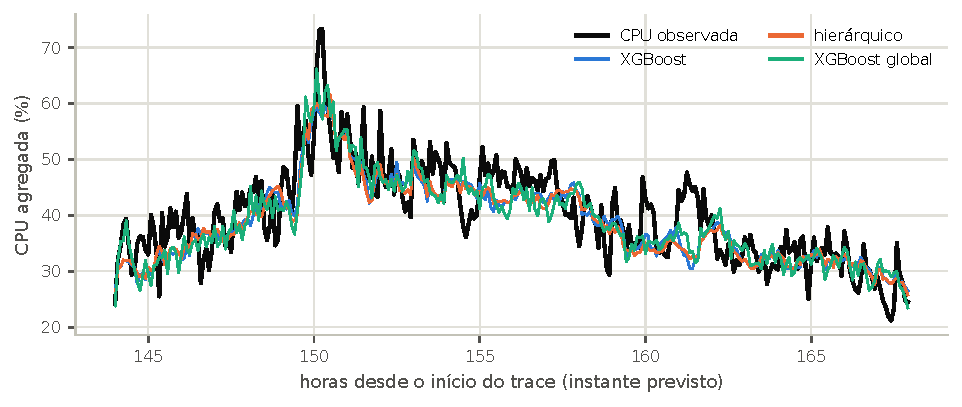
\includegraphics[width=0.95\textwidth]{figuras/serie_dia6_30min.pdf}\\
\textbf{\footnotesize Fonte: Autoria própria.}
\end{figure}

\subsection{Avaliação Estatística}
\label{sec:estatistica}

A Tabela~\ref{tab:comparacoes} apresenta as comparações pareadas. No teste final, o XGBoost superou a persistência com IC sem zero em 5 e 15~min; em 30~min, o IC conteve zero, e o ganho em 15~min deixou de ser significativo com blocos de 24 passos. Nenhuma diferença entre o híbrido e o XGBoost teve IC sem zero. As três redes pré-registradas foram piores que o XGBoost nos nove casos, mas, após Holm sobre as 93 comparações pré-registradas para o teste final, entre as das redes só a TCN em 30~min manteve significância.

\begin{table}[htbp]
\caption{Diferenças pareadas da perda (candidato $-$ referência) e IC de 95\% por \textit{block bootstrap}}
\label{tab:comparacoes}
\centering
\scriptsize
\setlength{\tabcolsep}{2.5pt}
\renewcommand{\arraystretch}{1.08}
\begin{tabularx}{\textwidth}{|P{5.4cm}|C|C|C|}
\hline
\textbf{Comparação} & \textbf{5 min} & \textbf{15 min} & \textbf{30 min} \\
\hline
\multicolumn{4}{|l|}{\textit{(a) Teste final de 24~h, MAE (p.p.), blocos de 1~h}} \\
\hline
XGBoost $-$ persistência & \textbf{$-$0,29 [$-$0,43; $-$0,08]} & \textbf{$-$0,85 [$-$1,52; $-$0,02]} & $-$1,00 [$-$1,90; 0,18] \\
Kalman + XGBoost $-$ XGBoost & $-$0,04 [$-$0,15; 0,05] & 0,07 [$-$0,28; 0,37] & $-$0,02 [$-$0,43; 0,35] \\
DLinear $-$ XGBoost & \textbf{0,21 [0,01; 0,38]} & \textbf{0,61 [0,17; 1,07]} & \textbf{0,81 [0,33; 1,27]} \\
TCN $-$ XGBoost & \textbf{0,36 [0,12; 0,60]} & \textbf{0,86 [0,34; 1,35]} & \textbf{1,04 [0,46; 1,59]}$^\dagger$ \\
N-BEATSx $-$ XGBoost & \textbf{0,74 [0,23; 1,27]} & \textbf{1,34 [0,47; 2,13]} & \textbf{0,92 [0,24; 1,49]} \\
\hline
\multicolumn{4}{|l|}{\textit{(b) Blocos diários, dias 3 a 6, bootstrap estratificado por dia (referência: XGBoost, salvo indicação)}} \\
\hline
H1: hierárquico (MAE) & $-$0,03 [$-$0,08; 0,02] & 0,00 [$-$0,07; 0,08] & $-$0,07 [$-$0,16; 0,02] \\
H2: XGBoost global (MAE) & 0,06 [$-$0,07; 0,18] & $-$0,01 [$-$0,13; 0,13] & 0,00 [$-$0,13; 0,15] \\
H3: combinação por regime (MAE) & $-$0,02 [$-$0,08; 0,04] & \textbf{$-$0,13 [$-$0,24; $-$0,02]}$^{m}$ & $-$0,04 [$-$0,18; 0,11] \\
H4: peso nas subidas (viés nos picos) & $-$0,02 [$-$0,04; 0,07] & \textbf{$-$0,51 [$-$0,82; $-$0,22]}$^{\dagger}$ & \textbf{$-$0,53 [$-$0,85; $-$0,08]} \\
H5: ACI $-$ conformal estático (\textit{interval score}) & \textbf{$-$0,62 [$-$1,41; $-$0,01]}$^{m}$ & $-$0,49 [$-$1,86; 0,72] & não calculável \\
H6: rota por grupo $-$ rota da média (energia, Wh) & \textbf{$-$198 [$-$266; $-$131]}$^{m\dagger}$ & \textbf{$-$359 [$-$560; $-$128]}$^{m}$ & \textbf{$-$647 [$-$1.118; $-$108]}$^{m}$ \\
H8a: DLinear normalizado $-$ sem normalização (MAE) & $-$0,04 [$-$0,09; 0,01] & $-$0,08 [$-$0,18; 0,04] & \textbf{$-$0,42 [$-$0,66; $-$0,18]}$^{m\dagger}$ \\
H8b: XGBoost com peso de recência (MAE) & $-$0,05 [$-$0,12; 0,01] & \textbf{0,14 [0,03; 0,25]}$^{p}$ & 0,14 [$-$0,03; 0,29] \\
H8c: XGBoost sem calendário (MAE) & 0,05 [$-$0,06; 0,12] & \textbf{0,36 [0,12; 0,51]}$^{p\dagger}$ & \textbf{0,55 [0,23; 0,76]}$^{p\dagger}$ \\
\hline
\end{tabularx}
\\[0.2cm]
\textbf{\footnotesize Fonte: Autoria própria. Negrito: IC sem zero. $^{m}$/$^{p}$: decisão pré-registrada ``melhor''/``pior'' (IC sem zero e mesmo sentido em pelo menos 3 de 4 dias). $^\dagger$: $p$ de Holm abaixo de 0,05. H4 em 15 e 30~min teve só 2 de 4 dias favoráveis. H5 em 30~min: limite infinito em 63 origens.}
\end{table}

Nos blocos diários, das 26 comparações primárias calculáveis, seis favoreceram o candidato e três a referência. Sobreviveram a Holm a rota de energia por grupo em 5~min, o DLinear normalizado em 30~min e a piora sem calendário em 15 e 30~min. Hierárquico e global não se distinguiram do XGBoost. Na grade completa de 90 configurações hierárquicas fixas, 87 tiveram MAE menor que o do XGBoost (até $-0{,}09$~p.p.), mas o candidato escolhido na validação interna mudou de configuração em quase todo bloco. No modelo global, aumentar a amostra de 256 para 4.015 máquinas não reduziu o erro; com correlação média de cerca de 0,6 entre as máquinas, o tamanho efetivo estimado por efeito de desenho foi de 645 a 1.434 observações por bloco, contra centenas de milhares de exemplos. Por máquina, o modelo global foi melhor que a persistência da própria máquina em 82\% a 93\% dos máquina-dias, ganho que não apareceu no agregado.

A Figura~\ref{fig:vies} mostra o diagnóstico que motivou H8a. Nos cinco blocos diários, o viés em 30~min do XGBoost, do DLinear e da TCN acompanhou o deslocamento de nível entre bloco e treino com correlação de 0,99: os modelos subestimam quando o bloco está acima do treino e superestimam no único dia abaixo dele. Com a normalização por janela, a correlação caiu para 0,56 (DLinear) e 0,23 (TCN). As redes normalizadas, porém, continuaram não distinguíveis do XGBoost nas nove comparações exploratórias.

\begin{figure}[htb]
\centering
\caption[Viés e deslocamento de nível]{Viés em 30~min por bloco diário contra o deslocamento de nível entre bloco e treino, com a correlação $r$ nos cinco blocos (dias 3 a 7)}
\label{fig:vies}
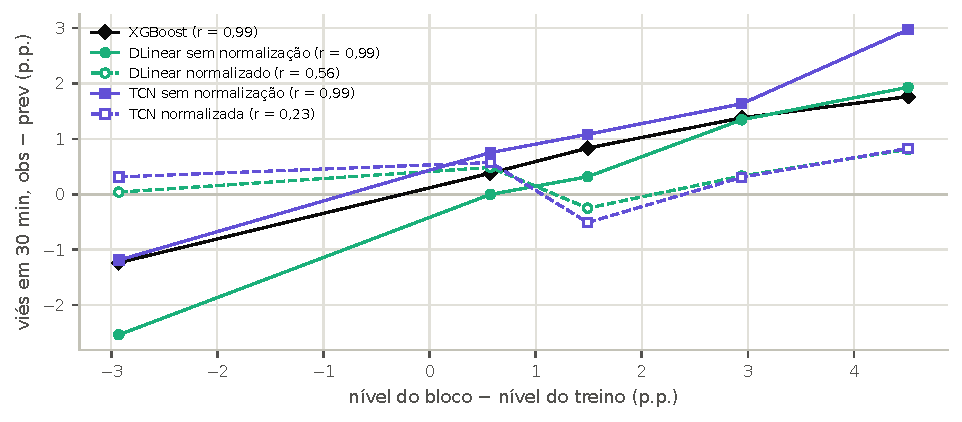
\includegraphics[width=0.95\textwidth]{figuras/vies_deslocamento.pdf}\\
\textbf{\footnotesize Fonte: Autoria própria.}
\end{figure}

\subsection{Análise dos Picos}
\label{sec:picos}

Todos os modelos subestimaram os picos (Figura~\ref{fig:picos}). No teste final, o viés nos picos em 30~min foi de $+4{,}4$~p.p.\ no XGBoost, $+4{,}8$ no híbrido e de $+6{,}0$ a $+9{,}0$ nas redes DLinear, TCN e N-BEATSx; entre 60\% e 94\% dos picos foram subestimados, conforme o modelo. O maior erro absoluto em 30~min foi de 25,8~p.p.\ no XGBoost, contra 38,3 na persistência. Em 5~min, a persistência teve o menor viés nos picos ($+2{,}4$), mas o maior MAE geral.

\begin{figure}[htb]
\centering
\caption[Subestimação nos picos]{Viés nos picos, fração de picos subestimados e distribuição do erro em 30~min no teste final (picos: CPU $\geq$ 50,4\%)}
\label{fig:picos}
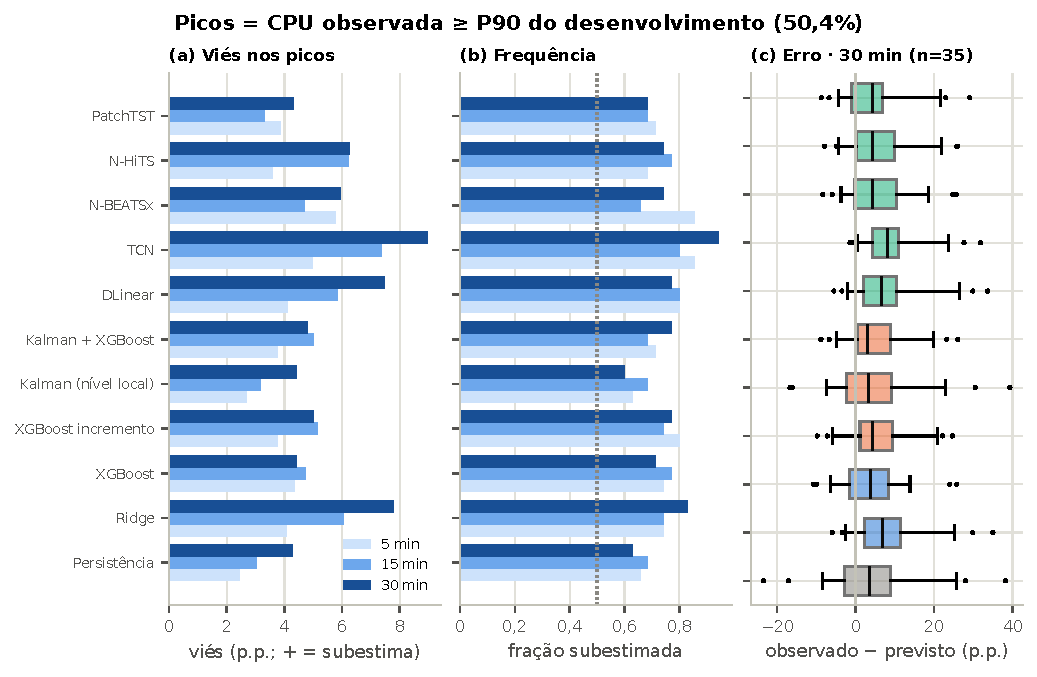
\includegraphics[width=\textwidth]{figuras/subestimacao_picos.pdf}\\
\textbf{\footnotesize Fonte: Autoria própria.}
\end{figure}

Nos blocos diários, o peso nas subidas (H4) reduziu o viés nos picos em 0,5~p.p.\ em 15 e 30~min (Tabela~\ref{tab:comparacoes}), mas só nos dias 3 e 4, em que a regra escolheu $\lambda = 3$; nos dias 5 e 6, a restrição de MAE ou a ausência de picos na validação interna manteve $\lambda = 0$. Com $\lambda = 3$ fixo, o viés nos picos caiu de 0,7 a 0,8~p.p., o MAE geral subiu de 0,15 a 0,32~p.p., e os episódios de falso alarme passaram de 0 para 6 a 8 em 26 eventos; de 80\% a 88\% dos picos continuaram subestimados. O peso desloca a previsão para cima, mas não antecipa a forma do pico.

\subsection{Previsão Probabilística}
\label{sec:probabilistica}

No teste final, o limite Q95 cobriu de 0,889 a 0,899 das origens, e a calibração conformal estática elevou a cobertura para 0,910 a 0,927, ainda abaixo do nominal de 0,95; nos picos, a cobertura ficou entre 0,63 e 0,71. Nos dias 3 a 6, o conformal estático cobriu 0,907, 0,888 e 0,854 em 5, 15 e 30~min, e só 0,49 dos picos em 30~min. A calibração adaptativa (ACI, $\gamma = 0{,}005$) cobriu 0,957, 0,947 e 0,947, e 0,88 dos picos em 30~min, com intervalos de 1,7 a 4,5~p.p.\ mais largos; a janela móvel de 288 escores cobriu de 0,928 a 0,939, e a predição conformal sequencial por regressão quantílica (SPCI) ficou abaixo do estático. A alta volatilidade foi o regime de pior cobertura em todos os métodos.

\subsection{Estimativa Energética}
\label{sec:energia}

A Tabela~\ref{tab:energia} resume a energia de TI modelada. No bloco (a), a curva foi aplicada à CPU agregada, como um servidor médio do 2288H V5: a energia de referência em 24~h foi de 6.530~Wh por servidor ($r = 1{,}4$). O erro relativo por janela ficou entre 2,3\% e 3,7\% em 5~min e entre 3,8\% e 6,1\% em 30~min. No acumulado de 24~h, porém, a ordem mudou: persistência e Kalman, sem viés, ficaram em $+0{,}8\%$ e $+0{,}1\%$, enquanto os modelos aprendidos, que subestimam a CPU, acumularam de $-0{,}9\%$ a $-3{,}7\%$. O erro de potência é quase linear no erro de CPU, cerca de 4,1~W por ponto percentual, e o erro relativo mudou pouco com $r$.

\begin{table}[htbp]
\caption{Erro de energia de TI modelada ($r = 1{,}4$, servidor substituto 2288H V5)}
\label{tab:energia}
\centering
\footnotesize
\setlength{\tabcolsep}{3pt}
\renewcommand{\arraystretch}{1.05}
\begin{tabularx}{\textwidth}{|P{5.0cm}|C|C|C|C|}
\hline
\multicolumn{5}{|l|}{\textit{(a) Teste final de 24~h, curva aplicada à CPU agregada (por servidor)}} \\
\hline
\textbf{Modelo} & \textbf{Erro rel. 5 min} & \textbf{Erro rel. 30 min} & \textbf{Viés 30 min (Wh)} & \textbf{Acumulado 24~h} \\
\hline
Persistência & 2,57\% & 5,20\% & $-$0,24 & $+$0,76\% \\
XGBoost & 2,35\% & 3,78\% & $-$1,91 & $-$1,24\% \\
Kalman + XGBoost & 2,33\% & 4,03\% & $-$1,86 & $-$1,07\% \\
Kalman (nível local) & 2,50\% & 4,79\% & $-$0,26 & $+$0,09\% \\
DLinear & 2,48\% & 4,81\% & $-$2,58 & $-$1,76\% \\
N-BEATSx & 3,67\% & 6,07\% & $-$5,03 & $-$3,65\% \\
\hline
\multicolumn{5}{|l|}{\textit{(b) Blocos diários, dias 3 a 6, soma das máquinas; erro total relativo por janela}} \\
\hline
\textbf{Modelo e rota} & \textbf{5 min} & \textbf{15 min} & \textbf{30 min} & \textbf{Agregação 30 min} \\
\hline
Persistência, média da frota & 2,90\% & 4,60\% & 5,44\% & $+$1,21\% \\
XGBoost, média da frota & 2,76\% & 4,00\% & 4,31\% & $+$1,21\% \\
Hierárquico, média do grupo & 2,49\% & 3,82\% & 4,13\% & $+$0,51\% \\
XGBoost global, por máquina & 2,54\% & 3,70\% & 3,96\% & 0 \\
\hline
\end{tabularx}
\\[0.2cm]
\textbf{\footnotesize Fonte: Autoria própria. Estimativa paramétrica, não medição. Erro rel.: média de $|E_{\mathrm{proj}} - E_{\mathrm{ref}}|/E_{\mathrm{ref}}$ por origem. Agregação: parcela da Equação~\eqref{eq:decomposicao} em \% da referência.}
\end{table}

O bloco (b) mostra o efeito da agregação. Aplicar a curva à CPU média superestimou a energia de referência por máquina em 1,21\% com $r = 1{,}4$ e 1,68\% com $r = 1{,}8$; com $r = 1$ as rotas coincidem, porque a curva é linear (Figura~\ref{fig:energia}a). O mesmo efeito já tinha sido medido de forma independente, sobre toda a série, como 3,2~W por servidor ($-1{,}2\%$ no sinal ``média das potências menos potência da média''). Na rota da média, a superestimação por agregação se soma a uma previsão que subestima a CPU, e as duas parcelas se compensam em parte. A rota por grupo reduziu o termo de agregação em cerca de 58\% e o erro total nos três horizontes (H6); com 16 grupos, o termo caiu para 0,26\%. A rota por máquina, com o modelo global, teve o menor erro total. A ordem dos métodos se manteve nos três servidores substitutos e no cenário sintético (Figura~\ref{fig:energia}b).

\begin{figure}[htb]
\centering
\caption[Energia de TI por rota]{Energia de TI modelada nos dias 3 a 6: (a) termo de agregação por rota e expoente $r$; (b) erro total por janela em 30~min por modelo, rota e servidor substituto}
\label{fig:energia}
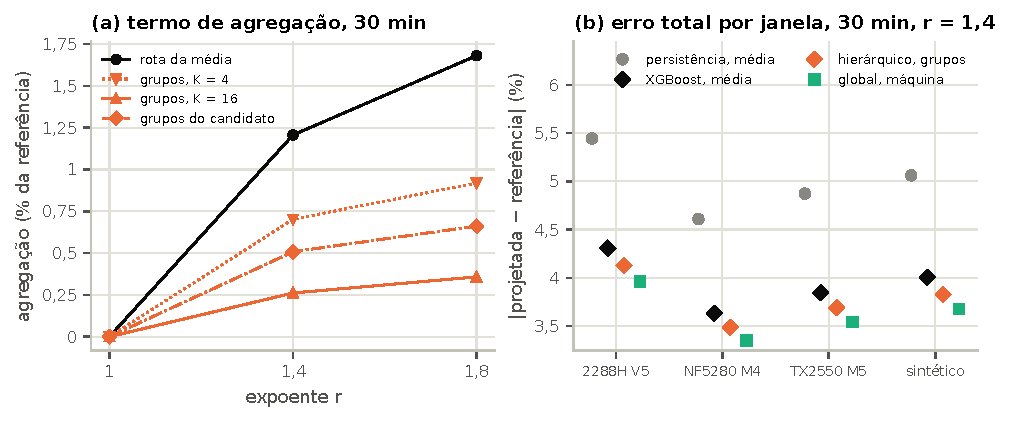
\includegraphics[width=\textwidth]{figuras/energia_rotas.pdf}\\
\textbf{\footnotesize Fonte: Autoria própria. Estimativa paramétrica em servidores substitutos.}
\end{figure}

%%%%%%%%%%%%%%%%%%%%%%%%%%%%%%%%%%%%%%%%%%%%%%%%%
%% 5. DISCUSSÃO
%%%%%%%%%%%%%%%%%%%%%%%%%%%%%%%%%%%%%%%%%%%%%%%%%

\section{Discussão}
\label{sec:discussao}

\textbf{Por que o XGBoost permaneceu competitivo.} O resultado medido é que nenhum modelo o superou com significância após Holm, em nenhuma das duas formas de avaliação. A interpretação apoiada pelos dados é que $u_t$, as médias móveis e o calendário já capturam quase toda a previsibilidade de curto prazo da série agregada: a autocorrelação é alta, as exógenas são redundantes e a importância TreeSHAP mostra o modelo passando de uma persistência corrigida, em 5~min, ao retorno ao padrão recente e diário, em 30~min. A retirada do calendário, que piorou o modelo com significância, confirma a utilidade dessa última componente.

\textbf{Como as redes se comportaram.} As redes não justificaram seu custo, embora pequeno (menos de 1~s por reajuste e cerca de 70~MB de memória de GPU). O diagnóstico de viés contra deslocamento de nível (Figura~\ref{fig:vies}) é compatível com previsões puxadas para o nível do treino, e a normalização por janela reduziu essa dependência. Como as redes normalizadas também não superaram o XGBoost, a desvantagem restante não pode ser atribuída só à mudança de nível; a hipótese mais simples é que, com cerca de 1.900 origens de treino, a arquitetura não tem estrutura a explorar além da que os atributos manuais já fornecem. Essa hipótese não foi testada diretamente.

\textbf{Estrutura por máquina.} A previsão hierárquica e o modelo global não trouxeram ganho distinguível no agregado. A correlação entre máquinas explica a ausência de efeito de escala: máquinas que oscilam juntas acrescentam pouca informação sobre a dinâmica do total. Os ganhos descritivos das configurações hierárquicas fixas (cerca de 2\%) são da ordem da variação entre dias e só poderiam ser confirmados num período não inspecionado. O valor da estrutura por máquina apareceu na energia, não na CPU.

\textbf{Picos, regimes e calibração.} O regime detectado no passado quase não antecipa a direção da variação: só 8\% das subidas e 4\% das quedas detectadas se confirmaram em 15~min, e o ganho da combinação veio de misturar previsores com erros pouco correlacionados, não da especialização. O peso nas subidas mostrou um compromisso, não um ganho de informação: menos subestimação nos picos ao custo de erro médio e alarmes falsos. A calibração adaptativa foi o refinamento de melhor relação custo-benefício: menos de 10~ms por bloco e cobertura próxima do nominal, compatível com escores de calibração que envelhecem quando o nível muda entre dias.

\textbf{Distribuição da carga e energia.} Como a curva de potência é côncava para $r > 1$, a distribuição da CPU entre as máquinas altera a energia estimada mesmo com a média conhecida. Um bom previsor da média da frota não basta para estimar energia sem viés; agrupar as máquinas remove a maior parte desse termo a custo baixo. No acumulado, o viés pesa mais que o erro por janela, e termos de sinais opostos podem se compensar num dia específico.

\textbf{Desempenho e complexidade.} O XGBoost com atributos de defasagem teve a melhor relação entre erro e custo (cerca de 0,06~s por reajuste em CPU). A média simples de previsores e a calibração adaptativa acrescentaram melhorias baratas. O modelo global custou de 30 a 80 vezes o tempo de ajuste e cerca de 4~GB de memória sem ganho no agregado, mas é o que permite a rota de energia por máquina.

\subsection{Limitações}
\label{sec:limitacoes}

\begin{itemize}
    \item \textbf{Energia modelada:} o \textit{trace} não tem medição elétrica; a energia é uma estimativa paramétrica em servidores substitutos do SPECpower\_ssj2008, um deles publicado em 2019, sem refrigeração. O PUE não foi calculado.
    \item \textbf{Reuso do teste:} o mesmo dia de teste foi inspecionado em mais de uma etapa da análise, e os dias 4 a 6 também já tinham servido de validação. Não há teste independente, e os resultados dos blocos diários são exploratórios.
    \item \textbf{Dados:} oito dias de um único cluster de 2018, sem sazonalidade semanal e com hardware desconhecido.
    \item \textbf{Dependência temporal:} o tamanho efetivo é menor que o número de origens; o \textit{block bootstrap} trata a dependência dentro de cada bloco, e a variação entre dias é estimada com $n = 4$.
    \item \textbf{População:} a população principal inclui uma máquina inativa e difere da coorte ativa em até 0,026~p.p.; as conclusões valem para a série agregada, não para máquinas individuais.
    \item \textbf{Referências metodológicas:} as fontes primárias dos métodos marcados no texto ainda precisam ser incluídas na bibliografia.
\end{itemize}

%%%%%%%%%%%%%%%%%%%%%%%%%%%%%%%%%%%%%%%%%%%%%%%%%
%% 6. CONCLUSÃO
%%%%%%%%%%%%%%%%%%%%%%%%%%%%%%%%%%%%%%%%%%%%%%%%%

\section{Conclusão}
\label{sec:conclusao}

Este trabalho respondeu à questão de pesquisa em duas partes. Na previsão de CPU, modelos de aprendizado de máquina superaram a persistência, de forma robusta em 5~min ($-0{,}29$~p.p.\ de MAE no teste) e com ganho de 13\% a 19\% em 15 e 30~min, menos robusto estatisticamente. O XGBoost com defasagens, médias móveis e calendário teve o melhor equilíbrio entre desempenho e custo; o híbrido Kalman + XGBoost e a média simples de previsores ficaram no mesmo nível, sem diferença significativa. Cinco redes neurais, a previsão hierárquica, o modelo global e a combinação por regime não o superaram com significância. Na energia, o erro de CPU se traduziu em 2,3\% a 6,1\% de erro de energia de TI modelada por janela, com o viés dominando o acumulado.

A avaliação por blocos diários acrescentou três contribuições: o diagnóstico de que o viés dos modelos acompanha o deslocamento de nível entre treino e avaliação, a correção da cobertura dos limites superiores por calibração adaptativa e a quantificação do efeito de agregação na energia, que superestima a energia modelada em cerca de 1,2\% e é reduzido pela modelagem por grupos de máquinas. Os picos continuam sendo o ponto fraco: todos os modelos os subestimam, e reduzir essa subestimação custa erro médio e alarmes falsos. No plano metodológico, o trabalho oferece um protocolo de validação temporal com purga, pré-registro e inferência por \textit{block bootstrap} que distingue efeitos estatisticamente sustentados de diferenças de ruído.

Os resultados apoiam o planejamento energético como estimativa, não como medição, e não demonstram redução de consumo em um \textit{datacenter} real. Como trabalhos futuros, propõem-se: confirmar os candidatos avaliados nos blocos diários num período ou \textit{trace} não inspecionado; calibrar o modelo de potência em hardware com medição elétrica, condição para discutir PUE com dados reais; estimar a incerteza da energia acumulada com modelos de trajetória conjunta; e tratar a detecção de picos como classificação com custo explícito de falso alarme.

%%%%%%%%%%%%%%%%%%%%%%%%%%%%%%%%%%%
%% FIM DO TEXTO
%%%%%%%%%%%%%%%%%%%%%%%%%%%%%%%%%%%

\newpage
\singlespacing
\bibliographystyle{abntex2-alf}
\bibliography{bibliografia}

\end{document}
